\documentclass[12pt,letterpaper, onecolumn]{exam}
\usepackage{amsmath}
\usepackage{amssymb}
\usepackage{graphicx}
\usepackage{setspace}
\usepackage{nicefrac}
\setcounter{MaxMatrixCols}{20}
\usepackage[lmargin=71pt, tmargin=1.2in]{geometry}  %For centering solution box
\lhead{Optimal Estimation}
\rhead{Noah Miller}
\thispagestyle{empty}   %For removing header/footer from page 1

\begin{document}

\begingroup
\centering
\LARGE Optimal Estimation\\
\LARGE Homework 1 \\[0.5em]
\large \today\\[0.5em]
\large Noah Miller\par
\large 903949330\par
\large MECH 7710\par
\endgroup
\pointsdroppedatright   %Self-explanatory
\printanswers
\renewcommand{\solution}{\noindent\textbf{Ans:}\enspace}   %Replace "Ans:" with starting keyword in solution box

\begin{questions}
	\question{Use the MATLAB function $>>conv$ to produce discrete probability functions (PDF’s) for
		throws of six dice as follows (note: this is effectively the sum of 6 random variables)}\\
	\begin{parts}
		\part{6 numbered: $1,\,2\,,3\,,4,\,5,\,6$}\\
		\solution
		We can write the probability density function of the first dice as equal to
		\[
			\begin{bmatrix}
				0 & \frac{1}{6} & \frac{1}{6} & \frac{1}{6} & \frac{1}{6} & \frac{1}{6} & \frac{1}{6} \\
			\end{bmatrix} \]
		where the first index $0$ has no probability of occurring because the dice cannot roll a 0. Plotting the convolutions for each dice is displayed below along with the mean and standard deviations for each case in the title. The mean and standard deviations for case were found using equations \ref{eq:1} and \ref{eq:2}.
		\begin{equation}\label{eq:1}
			\overline{x} = \sum x \cdot f_x^T
		\end{equation}
		\begin{equation}\label{eq:2}
			\sigma_x = \sqrt{(x - \overline{x})^2 \cdot f_x^T}
		\end{equation}
		\begin{figure}[!h]
			\centering
			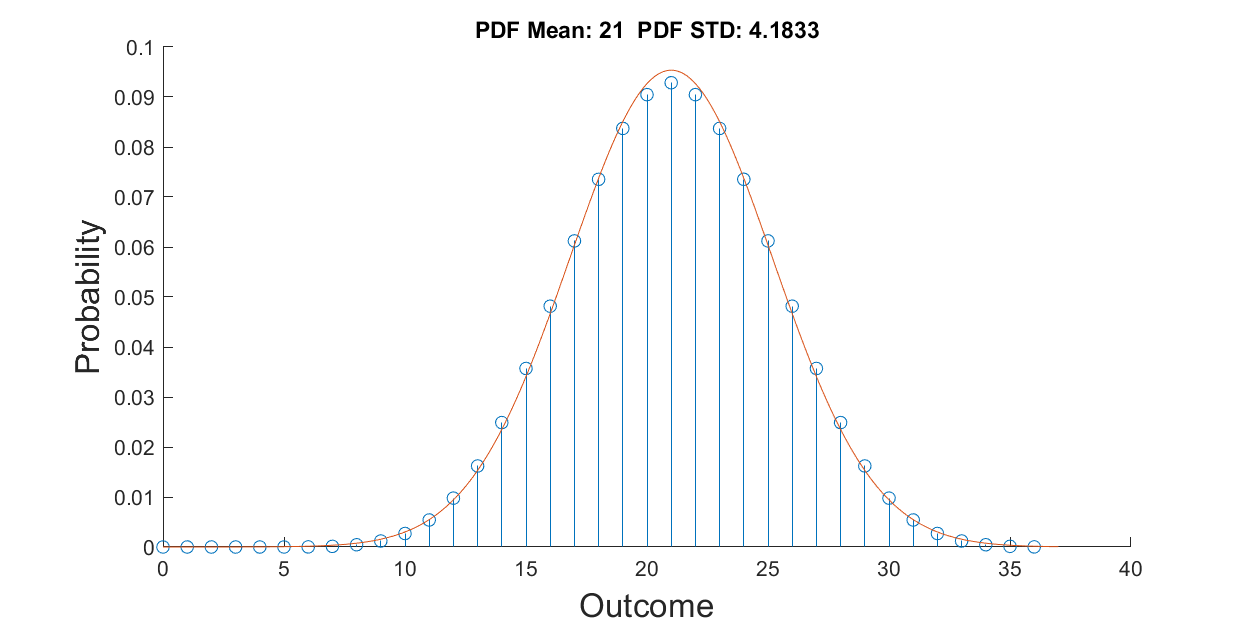
\includegraphics[width=.91\linewidth]{Q1_a.png}
		\end{figure}
		\clearpage
		\part{6 numbered: $4,\,5\,,6\,,7,\,8,\,9$}\\
		\solution
		\begin{figure}[!h]
			\centering
			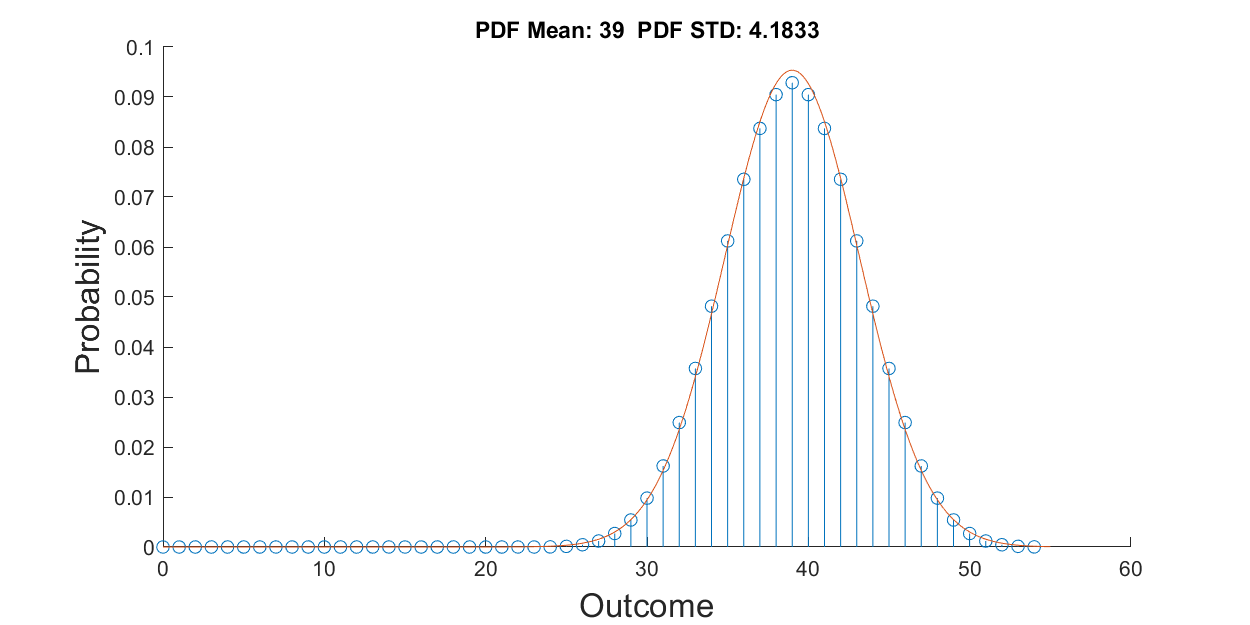
\includegraphics[width=.91\linewidth]{Q1_b.png}
		\end{figure}
		\part{6 numbered: $1,\,1\,,3\,,3,\,3,\,5$}\\
		\solution
		\begin{figure}[!h]
			\centering
			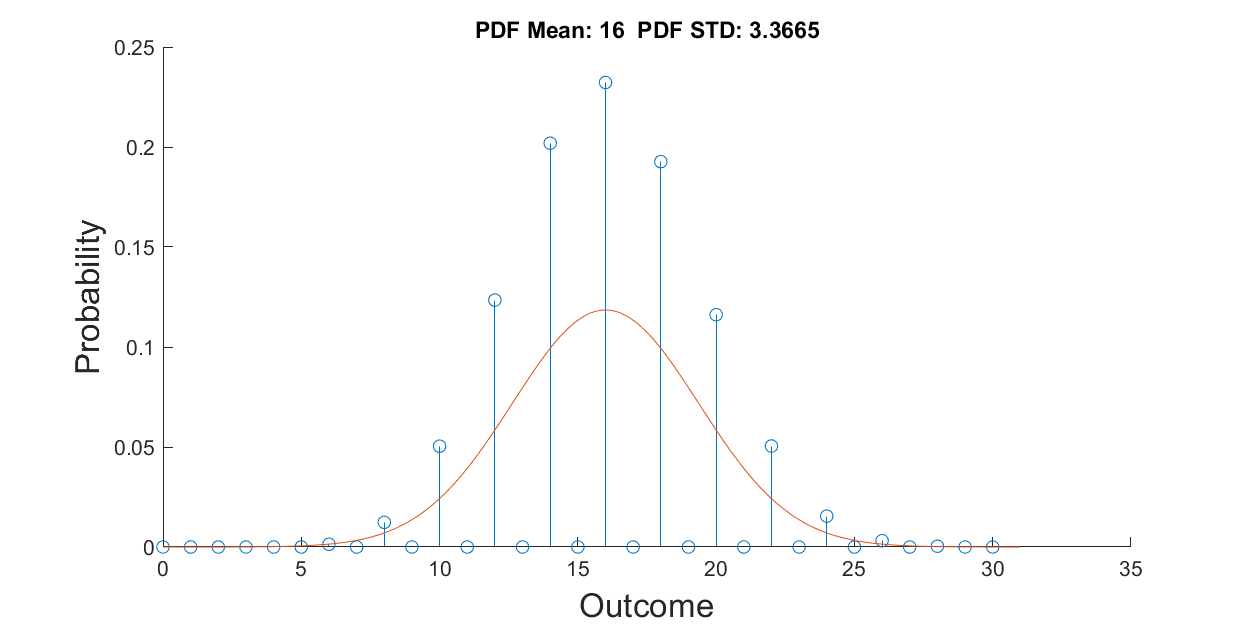
\includegraphics[width=.91\linewidth]{Q1_c.png}
		\end{figure}
		\clearpage
		\part{6 numbered: $1,\,2\,,3\,,4,\,5,\,6$ and 3 numbered: $1,\,1\,,3\,,3,\,3,\,5$}\\
		\solution
		\begin{figure}[!h]
			\centering
			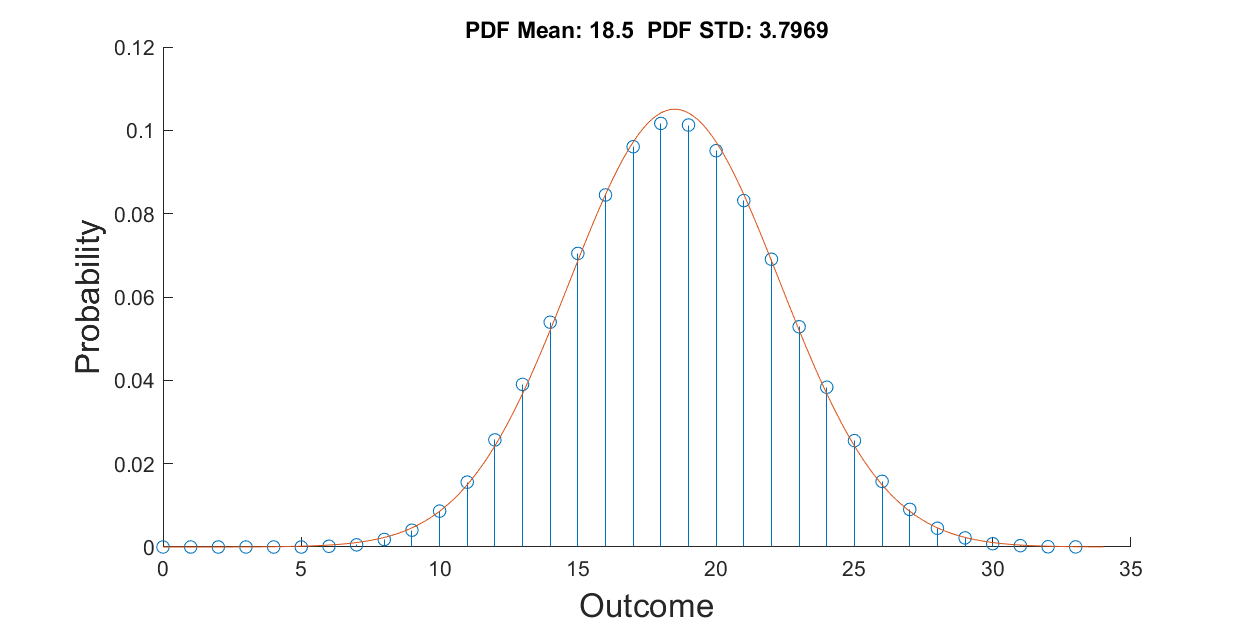
\includegraphics[width=.91\linewidth]{Q1_d.png}
		\end{figure}
	\end{parts}
	Check that the $\sum$PDF $= 1.0$\\
	Plot each PDF with a normal distribution plot of the same average and sigma.\\

	\textit{Note that even peculiar random distributions, taken in aggregate, tend to produce
		“normal” error distributions}
	\clearpage
	\question{What is the joint PDF for 2 fair dice $(\mathbf{X}_1, \mathbf{X}_2)$ (make this a $6\times6$ matrix with the indices equal to
		the values of the random variables). Note each row should add to the probability of the index
		for $x_1$ and each column to the probability of the index for $x_2$}\\
	\solution
	We define the rolls of two fair dice in a $6 \times 6$ matrix as follows:
	\begin{equation}
		PDF(\mathbf{X}_1, \mathbf{X}_2) =
		\frac{1}{36}
		\begin{bmatrix}
			1 & 1 & 1 & 1 & 1 & 1 \\
			1 & 1 & 1 & 1 & 1 & 1 \\
			1 & 1 & 1 & 1 & 1 & 1 \\
			1 & 1 & 1 & 1 & 1 & 1 \\
			1 & 1 & 1 & 1 & 1 & 1 \\
			1 & 1 & 1 & 1 & 1 & 1 \\
		\end{bmatrix}
	\end{equation}
	where the dice have the following numbered faces:
	\[\textbf{Dice 1:}
		\begin{bmatrix}
			1 & 2 & 3 & 4 & 5 & 6 \\
		\end{bmatrix} \]
	\[\textbf{Dice 2:}
		\begin{bmatrix}
			1 & 2 & 3 & 4 & 5 & 6 \\
		\end{bmatrix} \]
	\begin{parts}
		\part{What are
			\begin{subparts}
				\subpart{$E(\mathbf{X}_1)$}\\
				\solution
				\begin{equation}
					\begin{split}
						E(\mathbf{X}_1) & =\sum_{k = 1}^{6}\left(\mathbf{X}_1 f_{x_1}\left(\mathbf{x}_1 \right) \right)\\
						E(\mathbf{X}_1) & =
						\begin{bmatrix}
							1 & 2 & 3 & 4 & 5 & 6 \\
						\end{bmatrix}
						\begin{bmatrix}
							1/6 \\
							1/6 \\
							1/6 \\
							1/6 \\
							1/6 \\
							1/6 \\
						\end{bmatrix}\\
						E(\mathbf{X}_1) & = 3.5\\
					\end{split}
				\end{equation}
				\subpart{$E(\mathbf{X}_1 - E(\mathbf{X}_1))$}\\
				\solution
				\begin{equation}
					\begin{split}
						E(\mathbf{X}_1 - E(\mathbf{X}_1)) & = E(\mathbf{X}_1 - 3.5)\\
						E(\mathbf{X}_1 - E(\mathbf{X}_1)) & = E(\mathbf{X}_1) - 3.5\\
						E(\mathbf{X}_1 - E(\mathbf{X}_1)) & = 3.5 - 3.5\\
						E(\mathbf{X}_1 - E(\mathbf{X}_1)) & = 0\\
					\end{split}
				\end{equation}
				\clearpage
				\subpart{$E(\mathbf{X}_1^2)$}\\
				\solution
				\begin{equation}
					\begin{split}
						E(\mathbf{X}_1^2) & =
						\begin{bmatrix}
							1^2 & 2^2 & 3^2 & 4^2 & 5^2 & 6^2 \\
						\end{bmatrix}
						\begin{bmatrix}
							1/6 \\
							1/6 \\
							1/6 \\
							1/6 \\
							1/6 \\
							1/6 \\
						\end{bmatrix}\\
						E(\mathbf{X}_1^2) & =
						\begin{bmatrix}
							1 & 4 & 9 & 16 & 25 & 36 \\
						\end{bmatrix}
						\begin{bmatrix}
							1/6 \\
							1/6 \\
							1/6 \\
							1/6 \\
							1/6 \\
							1/6 \\
						\end{bmatrix}\\
						E(\mathbf{X}_1^2) & = 15.17\\
					\end{split}
				\end{equation}
				\subpart{$E((\mathbf{X}_1 - E(\mathbf{X_1}))^2)$}\\
				\solution
				\begin{equation}
					\begin{split}
						E\left((\mathbf{X}_1 - E(\mathbf{X}_1))^2\right) & = E\left((\mathbf{X}_1 - 3.5)^2\right)\\
						E\left((\mathbf{X}_1 - E(\mathbf{X}_1))^2\right) & =
						\begin{bmatrix}
							\frac{1}{6} & \frac{1}{6} & \frac{1}{6} & \frac{1}{6} & \frac{1}{6} & \frac{1}{6} \\
						\end{bmatrix}
						\left(
						\begin{bmatrix}
								1 \\
								2 \\
								3 \\
								4 \\
								5 \\
								6 \\
							\end{bmatrix} -
						\begin{bmatrix}
								3.5 \\
								3.5 \\
								3.5 \\
								3.5 \\
								3.5 \\
								3.5 \\
							\end{bmatrix}
						\right)^2\\
						E\left((\mathbf{X}_1 - E(\mathbf{X}_1))^2\right) & = 2.92\\
					\end{split}
				\end{equation}
				\subpart{$E(((\mathbf{X}_1 - E(\mathbf{X}_1))\cdot(\mathbf{X}_2 - E(\mathbf{X}_2)))$}\\
				\solution
				Because the rolls of two different, but equal and fair dice are independent events, we can say the expectation of their combined rolls are uncorrelated and thusly 0.
				\begin{equation}
					\begin{split}
						E(((\mathbf{X}_1 - E(\mathbf{X}_1))\cdot(\mathbf{X}_2 - E(\mathbf{X}_2))) & = 0\\
					\end{split}
				\end{equation}

			\end{subparts}}
		\part{Form the covariance matrix for $x_1$ and $x_2$}\\
		\solution
		We can find the diagonal indices of the $x_1$,$x_2$ covariance matrix following a similar fashion that was done in class.
		\begin{equation}\begin{split}\label{eq:9}
				P_{11} & = E(x_1^2) - E(x_1)^2\\
				P_{11} & = 15.17 - 3.5^2\\
				P_{11} & = 2.917\\
			\end{split}\end{equation}
		\begin{equation}\begin{split}
				P_{22} & = E(x_2^2) - E(x_2)^2\\
				P_{22} & = 15.17 - 3.5^2\\
				P_{22} & = 2.917\\
			\end{split}\end{equation}
		As we stated earlier, $x_1$ and $x_2$ are independent and uncorrelated, so the off-diagonal indices of the covariance matrix are simply 0, Giving us
		\[\mathbf{P} =
			\begin{bmatrix}
				2.917 & 0     \\
				0     & 2.917 \\
			\end{bmatrix}.\]

		\part{Now find the PDF matrix for the variables $v_1 = x_1$ and $v_2 = x_1 + x_2$.}\\
		\solution
		\begin{equation}
			\begin{split}
				PDF(v_1,v_x) & = \frac{1}{36}\cdot
				\begin{bmatrix}
					1 & 1 & 1 & 1 & 1 & 1 & 0 & 0 & 0 & 0 & 0 \\
					0 & 1 & 1 & 1 & 1 & 1 & 1 & 0 & 0 & 0 & 0 \\
					0 & 0 & 1 & 1 & 1 & 1 & 1 & 1 & 0 & 0 & 0 \\
					0 & 0 & 0 & 1 & 1 & 1 & 1 & 1 & 1 & 0 & 0 \\
					0 & 0 & 0 & 0 & 1 & 1 & 1 & 1 & 1 & 1 & 0 \\
					0 & 0 & 0 & 0 & 0 & 1 & 1 & 1 & 1 & 1 & 1 \\
				\end{bmatrix}\\
			\end{split}
		\end{equation}
		\part{Now what is the mean, $E(v_1 - E(v_1))$, rms, and variance of $v_1$}\\
		\solution

		The mean of $v_1$ is just the mean of $x_1$, which we already determined to be $3.5$.\\

		\begin{equation}
			E(v_1 - E(v_1)) = E(x_1 - E(x_1)) = 0
		\end{equation}\\

		The root mean square value for $v_1$ is just the square root of $E(x_1^2)$, or $3.89$.\\

		The variance of $v_1$ is just equation \ref{eq:9} and is equal to $2.917$.\\
		\part{what is the mean, $E(v_2 - E(v_2))$, rms, and variance of $v_2$}\\
		\solution

		The mean of $v_2$ is just double the mean of $x_1$ since $v_2$ is the sum of $x_1$ and $x_2$. This gives $v_2$ a mean of 7.\\

		\begin{equation}
			E(v_2 - E(v_2)) = 2\cdot E(x_1 - E(x_1)) = 0
		\end{equation}\\

		The root mean square value for $v_2$ is just double the square root of $E(x_1^2)$, or $7.41$.\\

		The variance of $v_1$ is just double equation \ref{eq:9} and is equal to $5.83$.\\
		\part{What is the new covariance matrix $P$.}\\
		\solution
		Using parts \textit{d} and \textit{e}, we can create a new covariance matrix, $\mathbf{P}$.
		\begin{equation}
			\mathbf{P} =
			\begin{bmatrix}
				2.917  & P_{21} \\
				P_{12} & 5.83   \\
			\end{bmatrix}
		\end{equation}
		In order to solve for the off-diagonals of the co-variance matrix we can solve
		\[E\left[(v_1 - \overline{v_1})(v_2 - \overline{v_2}) \right] \]
		Filling out what we already know simplifies this problem greatly.
		\begin{equation}
			\begin{split}
				E\left[(v_1 - \overline{v_1})(v_2 - \overline{v_2}) \right] & = E\left[(v_1 - 3.5)(v_2 - 7) \right]\\
				E\left[(v_1 - \overline{v_1})(v_2 - \overline{v_2}) \right] & = E\left[v_1v_2 - 7v_1 - 3.5v_2 + 24.5\right]\\
				v_2 & = x_1 + x_2\\
				v_1 & = x_1\\
				E\left[(v_1 - \overline{v_1})(v_2 - \overline{v_2}) \right] & = E\left[x_1^2 + x_1x_2 - 7x_1 - 3.5(x_1 + x_2) + 24.5\right]\\
				E\left[(v_1 - \overline{v_1})(v_2 - \overline{v_2}) \right] & = 15.17 + 12.25 - 24.5 - 12.25 - 12.25 + 24.5\\
				E\left[(v_1 - \overline{v_1})(v_2 - \overline{v_2}) \right] & = 2.92\\
			\end{split}
		\end{equation}
		This gives us a covariance matrix of:
		\begin{equation}
			\mathbf{P} =
			\begin{bmatrix}
				2.917 & 2.92 \\
				2.92  & 5.83 \\
			\end{bmatrix}
		\end{equation}
	\end{parts}
	\clearpage
	\question{Two random vectors $\mathbf{X}_1$ and $\mathbf{X_2}$ are uncorrelateed if \[E\{(\mathbf{X}_1 - \overline{\mathbf{X}}_1)(\mathbf{X}_2 - \overline{\mathbf{X}}_2) \} = 0 \]} Show that:
	\begin{parts}
		\part{Independent random vectors are uncorrelated}\\
		\solution
		In order to show that independent random vectors are uncorrelated, we must prove
		\[>>cov(\mathbf{X}_1,\mathbf{X}_2)\triangleq E\{(\mathbf{X}_1 - \overline{\mathbf{X}}_1)(\mathbf{X}_2 - \overline{\mathbf{X}}_2)\} = 0\]
		to be true. We start by expanding terms.
		\begin{equation}
			\begin{split}
				>>cov(\mathbf{X}_1,\mathbf{X}_2) & \triangleq E\{\mathbf{X}_1\mathbf{X}_2 - \mathbf{X}_1\overline{\mathbf{X}}_2 - \mathbf{X}_1\overline{\mathbf{X}}_1 + \overline{\mathbf{X}}_1\overline{\mathbf{X}}_2\}\\
				0 & = E\{\mathbf{X}_1\mathbf{X}_2\} - E\{\mathbf{X}_1\overline{\mathbf{X}}_2\} - E\{\mathbf{X}_2\overline{\mathbf{X}}_1\} + E\{\overline{\mathbf{X}}_1\overline{\mathbf{X}}_2\}\\
			\end{split}
		\end{equation}
		With the terms expanded, we can simplify each group and then combine like terms.
		\begin{equation}
			\begin{split}
				E\{\mathbf{X}_1\mathbf{X}_2\} & = E\{\mathbf{X}_1\}E\{\mathbf{X}_2\}\; = \;\overline{\mathbf{X}}_1\overline{\mathbf{X}}_2\\
				-E\{\mathbf{X}_1\overline{\mathbf{X}}_2\} & = -\overline{\mathbf{X}}_2E\{\mathbf{X}_1\} \; = \;-\overline{\mathbf{X}}_2\overline{\mathbf{X}}_1 \\
				-E\{\mathbf{X}_2\overline{\mathbf{X}}_1\} & = -\overline{\mathbf{X}}_1E\{\mathbf{X}_2\} \; = \;-\overline{\mathbf{X}}_1\overline{\mathbf{X}}_2 \\
				E\{\overline{\mathbf{X}}_1\overline{\mathbf{X}}_2\} & = \overline{\mathbf{X}}_1\overline{\mathbf{X}}_2\\
			\end{split}
		\end{equation}
		\begin{equation}
			\begin{split}
				0 & = \overline{\mathbf{X}}_1\overline{\mathbf{X}}_2 -\overline{\mathbf{X}}_2\overline{\mathbf{X}}_1 -\overline{\mathbf{X}}_1\overline{\mathbf{X}}_2 + \overline{\mathbf{X}}_1\overline{\mathbf{X}}_2\\
				0 & = 0\\
			\end{split}
		\end{equation}
		\part{Uncorrelated Gaussian random vectors are independent}\\
		\solution
		We know from class that a joint Gaussian distribution can be described by the following function (equation \ref{eq:20}).\\
		\begin{equation}\label{eq:20}
			f_{x,y}(x,y) = \frac{exp\left(\frac{-1}{2(1 - \rho_{12}^2)}\left(\frac{x^2}{\sigma_1^2} - 2\rho_{12}\frac{xy}{\sigma_1\sigma_2}+\frac{y^2}{\sigma^2_2}\right) \right)}{2\pi\sigma_1\sigma_2\sqrt{1 - \rho_{12}^2}}
		\end{equation}
	\end{parts}
	\clearpage
	\question{Consider a sequence created by throwing a pair of dice and summing the numbers which are $\{-2.5,-1.5,-0.5,0.5,1.5,2.5\}$. Call this $V_o(k)$.}
	\begin{parts}
		\part{What is the PDF?}\\
		\solution
		\part{What are the mean and variance of this sequence?}\\
		\solution

		If we generate a new random sequence \[V_N(k+1) = (1 - r)V_N(k) + rV_o(k)\]where $V_N(k)$ is serially-correlated (not white).
		\part{In steady state, what are the mean and variance of this new sequence $(V_N)$}\\
		\solution
		\part{What is the covariance function: $R(k) = E\{V_N(k)V_N(k-L)\}$}\\
		(Hint: $V_N(k)$ and $V_o(k)$ are uncorrelated).\\
		\solution
		\part{Are there any practical constraints on $r$?}\\
		\solution
	\end{parts}
	\clearpage
	\question{A random variable $x$ has a PDF given by:
		\[
			f_\mathbf{x}(x)=
			\begin{cases}
				0           & \text{if } x < 0           \\
				\frac{x}{2} & \text{if } 0 \leq x \leq 2 \\
				0           & \text{if } x \geq 2        \\
			\end{cases}
		\]}
	\begin{parts}
		\part{What is the mean of x?}\\
		\solution
		\part{what is the variance of x?}\\
		\solution
	\end{parts}
	\clearpage
	\question{Consider a normally distributed two-dimensional vector $\mathbf{X}$, with mean value zero and
		\[P_\mathbf{X} =
			\begin{bmatrix}
				2 & 1 \\
				1 & 4 \\
			\end{bmatrix} \]
	}
	\begin{parts}
		\part{Find the eigenvalues of $P_{\mathbf{X}}$}\\
		\solution
		\part{The likelihood ellipses are given by an equation of the form: $x^T P^{-1}_x x = c^2$. What are the principal axes in this case?}\\
		\solution
		\part{Plot the likelihood ellipses for $c = 0.25$, $1$, $1.5$}\\
		\solution
		\part{What is the probability of finding $\mathbf{X}$ inside each of these ellipses?}\\
		\solution
	\end{parts}
	\clearpage
	\question{Given $x \sim N(0,\sigma_x^2)$ and $y = 2x^2$}
	\begin{parts}
		\part{Find the PDF of $y$}\\
		\solution
		\part{Draw the PDFs of $x$ and $y$ on the same plot for $\sigma_x = 2.0$}\\
		\solution
		\part{How has the density function changed by this transformation?}\\
		\solution
		\part{Is $y$ a normal random variable?}\\
		\solution
	\end{parts}
\end{questions}
\end{document}